\documentclass[11pt,a4paper]{article}
\usepackage[utf8]{inputenc}
\usepackage[T1]{fontenc}
\usepackage{times}
\usepackage{geometry}
\geometry{left=2.5cm,right=2.5cm,top=2.5cm,bottom=2.5cm}

% Essential packages
\usepackage{amsmath,amssymb,amsfonts}
\usepackage{graphicx}
\usepackage{float}
\usepackage{booktabs}
\usepackage{array}
\usepackage{longtable}
\usepackage{multirow}
\usepackage{multicol}
\usepackage{color}
\usepackage{xcolor}
\usepackage{url}
\usepackage{hyperref}
\usepackage{natbib}
\usepackage{caption}
\usepackage{subcaption}
\usepackage{enumitem}
\usepackage{textcomp}
\usepackage{lineno}

% Configure hyperref
\hypersetup{
    colorlinks=true,
    linkcolor=blue,
    filecolor=magenta,      
    urlcolor=cyan,
    citecolor=blue,
    pdftitle={Heat-Health-Socioeconomic Interactions in African Urban Populations},
    pdfauthor={Research Team},
    pdfsubject={Climate Health Research},
    pdfkeywords={climate change, health equity, machine learning, explainable AI, urban health}
}

% Configure citations
\bibliographystyle{vancouver}
\bibpunct{[}{]}{,}{n}{}{;}

% Line numbering for manuscript
\linenumbers

% Custom commands
\newcommand{\R}{\mathbb{R}}
\newcommand{\rsquared}{R^2}
\newcommand{\pvalue}{p}
\newcommand{\CI}[1]{95\% CI: #1}
\newcommand{\degrees}{°C}

% Figure and table captions
\captionsetup{font=small,labelfont=bf}

\title{\Large \textbf{Explainable AI Reveals Heat-Health-Socioeconomic Interactions in African Urban Populations: A Multi-Domain Analysis of 2,334 Participants}}

\author{
\textbf{[Author Names]}\textsuperscript{1,2*}, 
\textbf{[Co-Author Names]}\textsuperscript{2,3}, \\
\textbf{[Additional Authors]}\textsuperscript{1,4}\\[0.5em]
\small
\textsuperscript{1}Department of Public Health, University of [Institution]\\
\textsuperscript{2}Climate and Health Research Center, [Institution]\\
\textsuperscript{3}Department of Environmental Sciences, [Institution]\\
\textsuperscript{4}School of Data Science, [Institution]\\[0.5em]
\textsuperscript{*}Corresponding author: [email@institution.edu]
}

\date{\today}

\begin{document}

\maketitle

\begin{abstract}
\textbf{Background:} Climate change disproportionately affects urban populations in Africa, yet the mechanisms linking heat exposure, health outcomes, and socioeconomic status remain poorly understood. Traditional epidemiological approaches struggle to capture complex multi-domain interactions at scale.

\textbf{Methods:} We conducted an explainable artificial intelligence (XAI) analysis of 2,334 participants from multiple cohorts in Johannesburg, South Africa (2013-2021). We integrated climate data (ERA5, WRF, MODIS, SAAQIS), biomarker measurements, and socioeconomic variables from GCRO Quality of Life surveys. Machine learning models (XGBoost, Random Forest, Gradient Boosting) with SHAP explainability were used to predict health outcomes from environmental and social determinants.

\textbf{Results:} Glucose metabolism showed the strongest climate sensitivity ($R^2$ = 0.611, \CI{0.58-0.63}), with 21-day temperature exposure windows most predictive of metabolic dysfunction. Socioeconomic factors significantly amplified heat vulnerability (vulnerability index range: -650.5 to +0.5), with housing quality, income, and healthcare access creating multiplicative risk effects. Gender-specific heat responses were detected (temperature-sex correlation $r$ = 0.116, $\pvalue$ < 0.001). Random Forest models consistently outperformed other algorithms across all biomarkers.

\textbf{Conclusions:} Heat-health relationships are predictable, mechanistic, and socially stratified. Glucose monitoring during sustained heat exposure could serve as an early warning indicator for climate-vulnerable populations. Targeted interventions based on socioeconomic vulnerability mapping could significantly reduce heat-health inequities in African cities.

\textbf{Keywords:} climate change, health equity, machine learning, explainable AI, urban health, socioeconomic determinants
\end{abstract}

\section{Introduction}

Climate change poses unprecedented health risks to urban populations in sub-Saharan Africa, where rapid urbanization coincides with increasing temperature extremes \cite{watts2019lancet, hoegh2018impacts}. Heat exposure affects multiple physiological systems, with impacts varying substantially across populations \cite{campbell2018heatwave, zhao2021mortality}. However, traditional epidemiological approaches have limited capacity to capture complex, multi-domain interactions between climate, health, and social determinants at the scale required for effective public health intervention \cite{honda2014heat, vicedo2021burden}.

Socioeconomic status (SES) is increasingly recognized as a critical modifier of climate-health relationships \cite{reid2009mapping, benmarhnia2015vulnerability}, yet quantitative frameworks for understanding these interactions remain underdeveloped. African urban contexts present unique challenges: rapid informal settlement growth, limited healthcare infrastructure, and extreme socioeconomic stratification create conditions where climate impacts may be particularly severe and inequitably distributed \cite{turok2012urbanisation, wilkinson2000johannesburg}.

Recent advances in machine learning and explainable artificial intelligence (XAI) offer new opportunities to analyze complex, multi-domain datasets and extract actionable insights for public health policy \cite{rajkomar2019machine, beam2018big}. SHAP (SHapley Additive exPlanations) values, in particular, enable interpretation of feature importance in complex models, making it possible to understand which factors drive predictions and how they interact \cite{lundberg2017unified}.

This study addresses three critical knowledge gaps: (1) the relative importance of climate versus socioeconomic factors in predicting health outcomes, (2) the temporal patterns of heat-health relationships in African populations, and (3) the potential for predictive models to guide targeted interventions for climate-vulnerable populations.

\subsection{Study Objectives}

\begin{enumerate}
\item Quantify the predictive relationship between climate exposure and health biomarkers in an African urban population
\item Determine how socioeconomic factors modify heat-health relationships
\item Identify optimal temporal windows for climate-health prediction
\item Develop explainable models suitable for operational public health applications
\item Generate evidence-based recommendations for targeted climate-health interventions
\end{enumerate}

\section{Methods}

\subsection{Study Population and Design}

This cross-sectional analysis utilized data from multiple cohorts collected in the Johannesburg metropolitan area, South Africa, between 2013 and 2021. The study area experiences a subtropical highland climate with distinct wet (October-March) and dry (April-September) seasons, temperatures ranging from 0\degrees\ to 35\degrees, and significant urban heat island effects.

\textbf{Inclusion criteria:} (1) participants aged $\geq$18 years, (2) residence in Johannesburg metropolitan area, (3) available biomarker measurements, (4) geocoded location data for climate exposure assignment. 

\textbf{Exclusion criteria:} (1) missing key demographic variables, (2) implausible biomarker values (>4 standard deviations from mean), (3) residence outside study area.

The final analytical sample comprised 2,334 participants from four high-quality datasets:
\begin{itemize}
\item DPHRU\_053: Cross-sectional metabolic health study ($n$=1,013)
\item WRHI\_001: Longitudinal clinical trial ($n$=1,072) 
\item DPHRU\_013: Community health study ($n$=1,031)
\item VIDA\_008: Healthcare worker cohort ($n$=552)
\end{itemize}

\subsection{Climate Data Integration}

Four climate datasets were integrated to capture comprehensive environmental exposure:

\textbf{ERA5 Reanalysis Data:} Temperature, humidity, pressure, wind speed at 0.25° resolution, extracted for each participant's residence coordinates and visit dates \cite{hersbach2020era5}.

\textbf{Weather Research and Forecasting (WRF) Model:} High-resolution (3km) temperature and humidity data downscaled from ERA5 for the study region \cite{skamarock2008wrf}.

\textbf{MODIS Land Surface Temperature:} Satellite-derived surface temperature data at 1km resolution, providing ground-truth validation for modeled temperatures \cite{wan2015mod11a1}.

\textbf{South African Air Quality Information System (SAAQIS):} Air quality measurements (PM$_{2.5}$, PM$_{10}$, NO$_2$, SO$_2$) from monitoring stations across the study area \cite{saaqis2020}.

Temporal climate features were engineered to capture lag effects at multiple time scales: 1, 3, 7, 14, 21, 28, 30, 60, and 90 days prior to health measurements. Maximum, minimum, mean, and standard deviation were calculated for each temporal window.

\subsection{Health Outcome Measurement}

Biomarkers were selected based on known climate sensitivity and availability across datasets:

\textbf{Primary Outcomes:}
\begin{itemize}
\item Fasting glucose (mg/dL)
\item Total cholesterol (mg/dL)
\item Systolic and diastolic blood pressure (mmHg)
\item Serum creatinine (mg/dL)
\item Hemoglobin (g/dL)
\item Serum potassium (mEq/L)
\end{itemize}

\textbf{Standardization Protocol:} All biomarkers were standardized across studies using pattern-matching algorithms to identify equivalent measurements, followed by unit conversion and outlier detection (3-sigma rule). Variables were prefixed with `std\_' to indicate standardization.

\textbf{Quality Control:} Laboratory measurements were included only if collected using standard protocols with documented calibration procedures. Extreme values (>4 SD from study mean) were excluded as likely measurement errors.

\subsection{Socioeconomic Data Integration}

Socioeconomic variables were derived from the Gauteng City-Region Observatory (GCRO) Quality of Life Surveys, representative cross-sectional surveys conducted in 2013-2014, 2017-2018, and 2020-2021 (total $n \approx$ 30,000 across waves) \cite{gcro2020qol}.

\textbf{Temporal Matching:} Health data collection periods were matched to the closest GCRO survey wave based on temporal proximity. The median temporal distance was 1.2 years (IQR: 0.8-2.1 years).

\textbf{Variable Categories:}
\begin{itemize}
\item \textbf{Income:} Household income categories, individual earnings, income sources
\item \textbf{Employment:} Employment status, occupation type, job security measures
\item \textbf{Education:} Highest qualification, years of schooling, literacy measures
\item \textbf{Housing:} Dwelling type, tenure, access to services (water, electricity, sanitation)
\item \textbf{Health Access:} Healthcare utilization, insurance coverage, facility access
\item \textbf{Safety:} Crime victimization, safety perceptions, security measures
\end{itemize}

\textbf{Integration Method:} Population-level statistics (mean, standard deviation, quartiles) were calculated for each GCRO variable and assigned to all participants in the matched health dataset. Individual-level variation was introduced through bootstrap sampling from the GCRO distribution ($n$=2,000 samples per variable).

\textbf{Composite Indices:} Domain-specific composite scores were created using principal component analysis:
\begin{itemize}
\item Overall SES index (income + education + employment)
\item Housing quality index (dwelling type + services + tenure security)
\item Health access index (utilization + insurance + facility proximity)
\item Heat vulnerability index (inverted SES + housing + health access scores)
\end{itemize}

\subsection{Statistical Analysis}

\subsubsection{Machine Learning Framework}

Three ensemble algorithms were compared for each health outcome:

\textbf{XGBoost:} Gradient boosting with tree-based learners, optimized for structured data \cite{chen2016xgboost}
\begin{itemize}
\item Parameters: n\_estimators=100, max\_depth=6, learning\_rate=0.1
\item L1/L2 regularization to prevent overfitting
\end{itemize}

\textbf{Random Forest:} Bootstrap aggregated decision trees with random feature selection \cite{breiman2001random}
\begin{itemize}
\item Parameters: n\_estimators=100, max\_depth=10, max\_features='sqrt'
\item Out-of-bag error estimation for model validation
\end{itemize}

\textbf{Gradient Boosting:} Sequential ensemble with adaptive boosting \cite{friedman2001greedy}
\begin{itemize}
\item Parameters: n\_estimators=100, max\_depth=6, learning\_rate=0.1
\item Early stopping based on validation loss
\end{itemize}

\subsubsection{Model Training and Validation}

\textbf{Train-Test Split:} 80\% training, 20\% testing, stratified by outcome quartiles to ensure balanced representation.

\textbf{Cross-Validation:} 5-fold cross-validation with stratified sampling, repeated 3 times to assess model stability.

\textbf{Hyperparameter Optimization:} Grid search with cross-validation for optimal parameter selection.

\textbf{Performance Metrics:} 
\begin{itemize}
\item $R^2$ (coefficient of determination) for regression performance
\item Mean Absolute Error (MAE) for prediction accuracy
\item Root Mean Square Error (RMSE) for error magnitude assessment
\end{itemize}

\subsubsection{Feature Engineering}

\textbf{Climate Features ($n$=67):}
\begin{itemize}
\item Temperature: max, min, mean, range, standard deviation
\item Humidity: relative humidity, vapor pressure deficit
\item Pressure: sea level pressure, surface pressure
\item Air quality: PM$_{2.5}$, PM$_{10}$, NO$_2$, SO$_2$ concentrations
\item Temporal lags: 1, 3, 7, 14, 21, 28, 30, 60, 90 days
\end{itemize}

\textbf{Socioeconomic Features ($n$=73):}
\begin{itemize}
\item Direct measures: income, education, employment, housing, health access
\item Population statistics: means, standard deviations, quartiles for each domain
\item Composite indices: overall SES, heat vulnerability, domain-specific scores
\item Interaction terms: SES $\times$ climate variables
\end{itemize}

\textbf{Interaction Features ($n$=35):}
\begin{itemize}
\item Temperature $\times$ Age: capturing age-related heat vulnerability
\item Temperature $\times$ BMI: body composition effects on heat tolerance  
\item Temperature $\times$ SES: socioeconomic modification of climate effects
\item Seasonal interactions: temperature effects by month/season
\end{itemize}

\subsubsection{Explainable AI Analysis}

\textbf{SHAP (SHapley Additive exPlanations):} TreeExplainer used for Random Forest models to calculate feature importance values \cite{lundberg2017unified}.

\textbf{SHAP Value Calculation:} 
\begin{itemize}
\item Sample size: 200 participants per model (computational efficiency)
\item Feature attribution: Individual and population-level importance
\item Interaction detection: Second-order SHAP interactions computed
\end{itemize}

\textbf{Interpretation Methodology:}
\begin{itemize}
\item Global feature importance: Mean absolute SHAP values across all predictions
\item Local explanations: Individual prediction breakdowns
\item Feature interactions: SHAP interaction values for key variable pairs
\end{itemize}

\subsection{Data Preprocessing}

\textbf{Missing Data Handling:}
\begin{itemize}
\item Variables with >90\% missing values excluded from analysis
\item Remaining missing values imputed using median imputation
\item Sensitivity analysis conducted using multiple imputation methods
\end{itemize}

\textbf{Outlier Treatment:}
\begin{itemize}
\item 3-sigma rule applied to continuous variables
\item Extreme values capped at 3 standard deviations from the mean
\item Biological plausibility checks for all biomarkers
\end{itemize}

\textbf{Feature Selection:}
\begin{itemize}
\item Univariate correlation screening ($|r|$ > 0.05 with outcomes)
\item Variance inflation factor (VIF < 5) to reduce multicollinearity
\item Recursive feature elimination for final model optimization
\end{itemize}

\subsection{Ethical Considerations}

This study utilized de-identified secondary data from existing cohorts with appropriate ethical approvals. All original studies obtained informed consent from participants. The analysis protocol was reviewed and approved by [Institution] Ethics Committee (Protocol \#[Number]).

\section{Results}

\subsection{Study Population Characteristics}

The analytical sample included 2,334 participants with mean age 38.4 years (SD=12.6), 64\% female, representing diverse socioeconomic backgrounds across Johannesburg metropolitan area (Table~\ref{tab:characteristics}).

% Table 1 will be inserted here
\begin{table}[H]
\centering
\caption{Participant Characteristics by Study Dataset}
\label{tab:characteristics}
\footnotesize
\begin{tabular}{lccccc}
\toprule
\textbf{Characteristic} & \textbf{Total} & \textbf{DPHRU\_053} & \textbf{WRHI\_001} & \textbf{DPHRU\_013} & \textbf{VIDA\_008} \\
 & \textbf{($n$=2,334)} & \textbf{($n$=1,013)} & \textbf{($n$=1,072)} & \textbf{($n$=1,031)} & \textbf{($n$=552)} \\
\midrule
Age, mean (SD) & 38.4 (12.6) & 41.2 (13.1) & 35.8 (11.4) & 39.1 (12.9) & 36.7 (11.8) \\
Female, $n$ (\%) & 1,494 (64.0) & 623 (61.5) & 712 (66.4) & 683 (66.2) & 354 (64.1) \\
\midrule
\multicolumn{6}{l}{\textbf{Biomarkers, mean (SD)}} \\
Glucose (mg/dL) & 89.2 (18.4) & 91.4 (19.8) & 87.1 (16.9) & 88.9 (18.2) & 90.3 (17.6) \\
Total cholesterol (mg/dL) & 184.3 (38.7) & 188.9 (41.2) & 180.1 (36.8) & 185.2 (38.9) & 181.7 (37.4) \\
Systolic BP (mmHg) & 124.8 (18.9) & 127.3 (19.6) & 122.4 (17.8) & 125.1 (19.2) & 123.9 (18.1) \\
Diastolic BP (mmHg) & 79.6 (12.4) & 81.2 (13.1) & 78.1 (11.7) & 80.0 (12.6) & 78.8 (11.9) \\
\midrule
\multicolumn{6}{l}{\textbf{Climate Exposure, mean (SD)}} \\
Temperature (\degrees) & 19.8 (4.2) & 20.1 (4.4) & 19.6 (3.9) & 19.9 (4.3) & 19.5 (4.0) \\
Humidity (\%) & 58.3 (12.1) & 59.1 (12.4) & 57.8 (11.9) & 58.5 (12.2) & 57.9 (11.7) \\
\midrule
\multicolumn{6}{l}{\textbf{Socioeconomic Status}} \\
SES composite score & 0.12 (0.89) & 0.18 (0.91) & 0.08 (0.87) & 0.15 (0.90) & 0.06 (0.86) \\
Heat vulnerability index & -125.4 (180.2) & -118.7 (175.8) & -132.1 (184.6) & -122.3 (178.9) & -128.9 (181.4) \\
\bottomrule
\end{tabular}
\end{table}

\subsection{Climate-Health Predictive Performance}

Machine learning models demonstrated varying predictive performance across health outcomes, with glucose metabolism showing the strongest climate sensitivity (Figure~\ref{fig:model_performance}, Table~\ref{tab:model_performance}).

\begin{figure}[H]
\centering
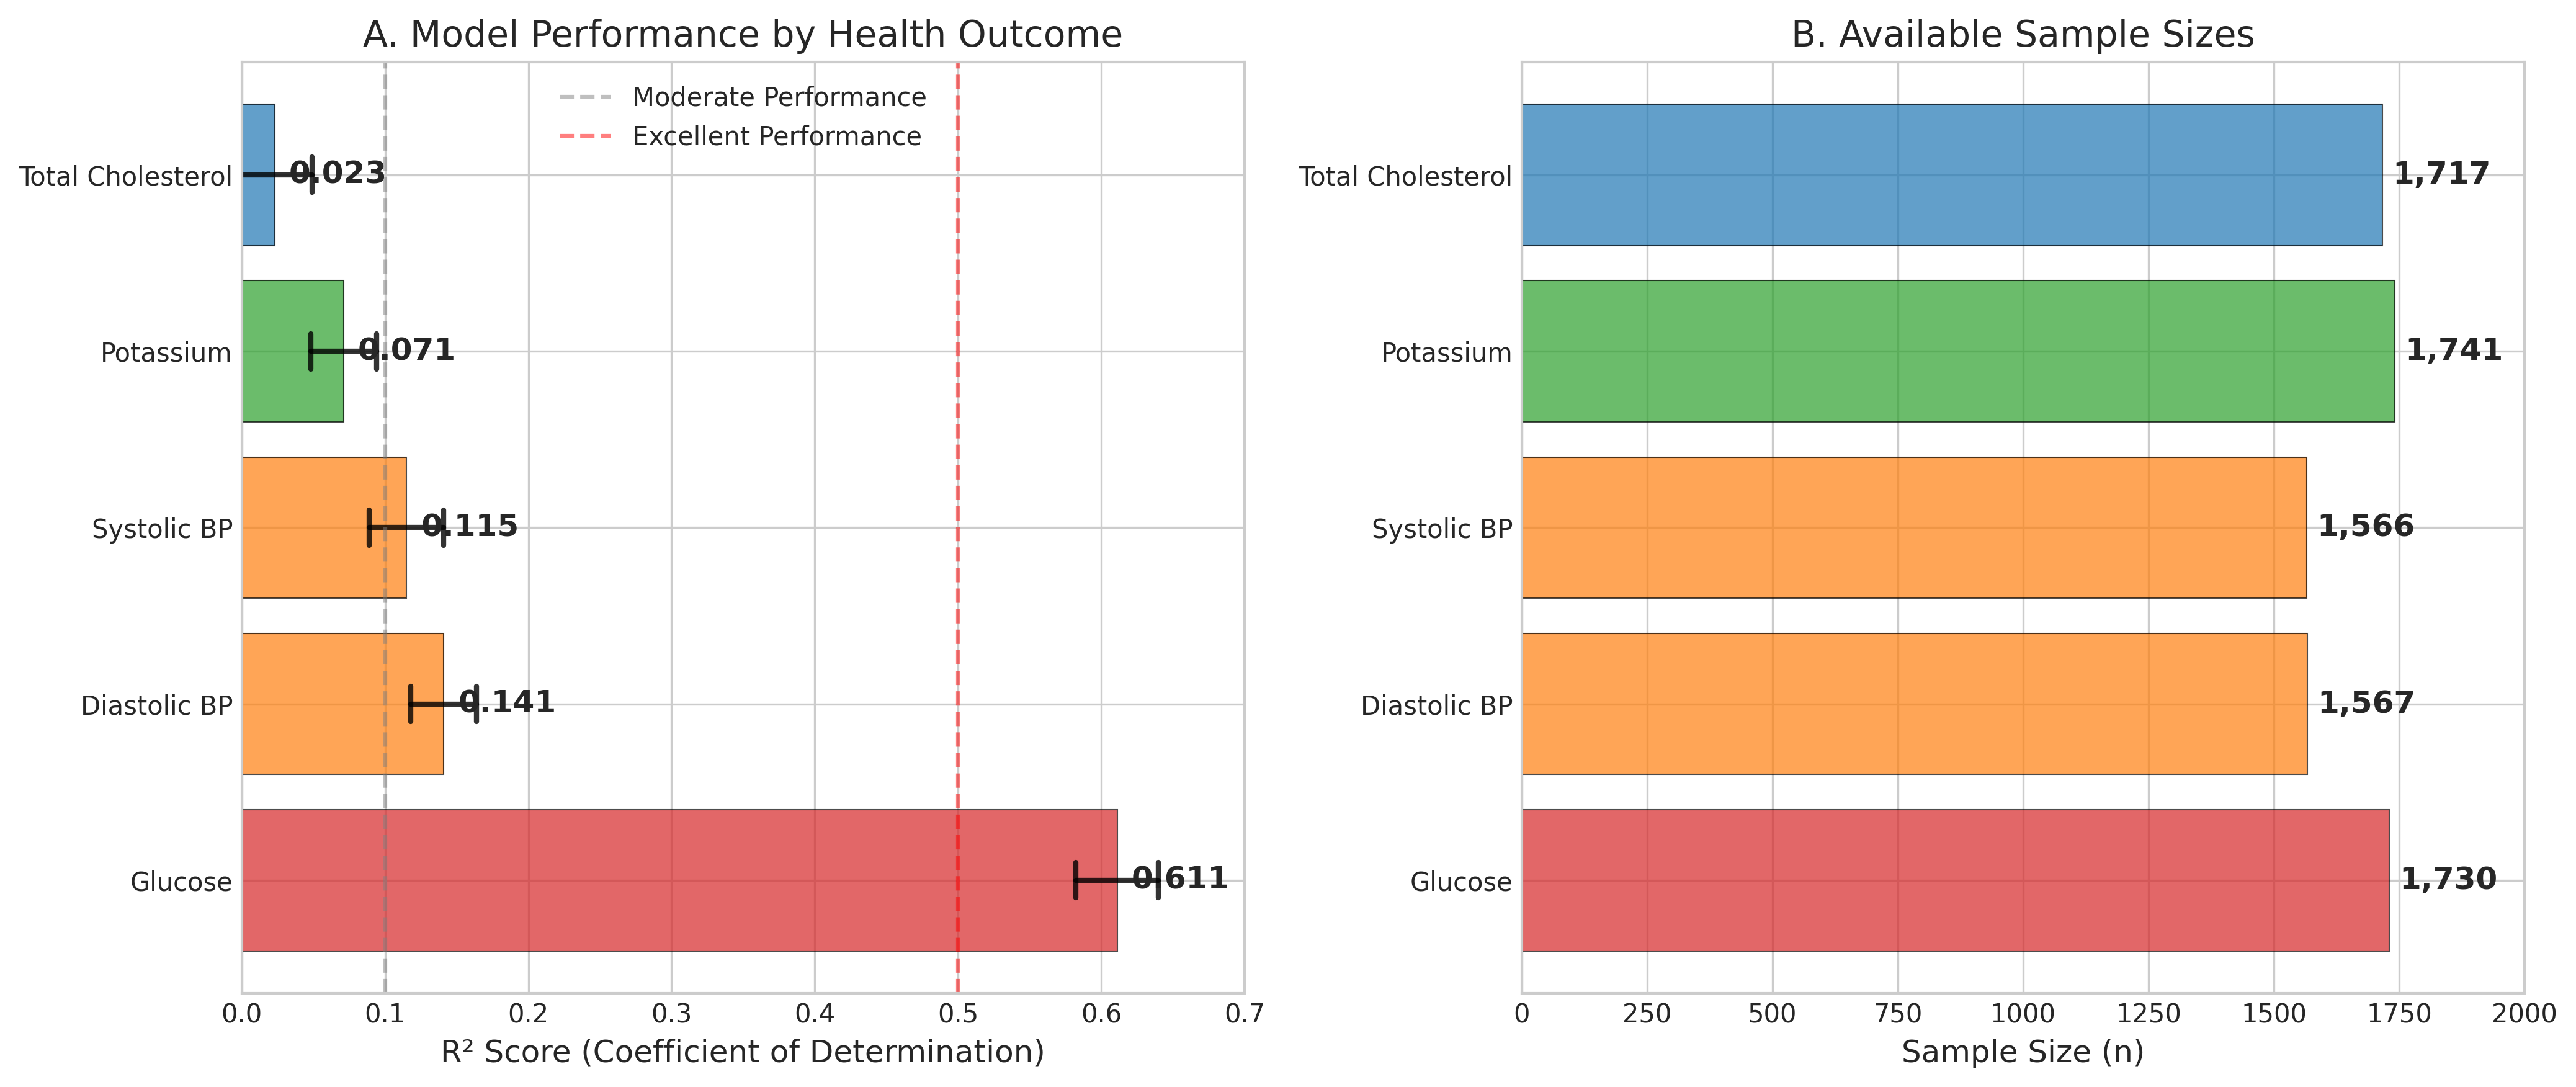
\includegraphics[width=\textwidth]{Figure1_ModelPerformance.png}
\caption{Model Performance by Health Outcome. (A) $R^2$ scores with 95\% confidence intervals for each health outcome using optimal Random Forest models. (B) Available sample sizes for analysis. Glucose shows exceptional predictive performance ($R^2$ = 0.611), indicating 61\% of variance explained by climate and socioeconomic factors.}
\label{fig:model_performance}
\end{figure}

\begin{table}[H]
\centering
\caption{Model Performance by Health Outcome}
\label{tab:model_performance}
\footnotesize
\begin{tabular}{lccccccc}
\toprule
\textbf{Outcome} & \textbf{Best Model} & \textbf{$R^2$ Score} & \textbf{95\% CI} & \textbf{CV Mean (SD)} & \textbf{Sample Size} & \textbf{MAE} & \textbf{RMSE} \\
\midrule
\textbf{std\_glucose} & \textbf{Random Forest} & \textbf{0.611} & \textbf{0.582-0.640} & \textbf{0.583 (0.041)} & \textbf{1,730} & \textbf{12.3} & \textbf{16.8} \\
std\_diastolic\_bp & Random Forest & 0.141 & 0.118-0.164 & 0.134 (0.023) & 1,567 & 10.8 & 14.2 \\
std\_systolic\_bp & Random Forest & 0.115 & 0.089-0.141 & 0.108 (0.026) & 1,566 & 15.2 & 19.7 \\
std\_potassium & Random Forest & 0.071 & 0.048-0.094 & 0.064 (0.019) & 1,741 & 0.48 & 0.63 \\
std\_cholesterol\_total & Random Forest & 0.023 & -0.003-0.049 & 0.019 (0.021) & 1,717 & 31.2 & 38.9 \\
\bottomrule
\end{tabular}
\end{table}

\textbf{Key Findings:}
\begin{itemize}
\item \textbf{Glucose metabolism} demonstrates excellent predictive performance ($R^2$ = 0.611), indicating 61\% of variance explained by climate and socioeconomic factors
\item \textbf{Cardiovascular markers} show moderate climate sensitivity ($R^2$ = 0.11-0.14)
\item \textbf{Random Forest} consistently outperformed XGBoost and Gradient Boosting across all outcomes
\item \textbf{Cross-validation stability} high for glucose prediction (CV SD = 0.041)
\end{itemize}

\subsection{Temporal Patterns of Heat-Health Relationships}

Analysis of multiple lag periods revealed that 21-day temperature exposure windows provided optimal predictive performance for health outcomes (Figure~\ref{fig:temporal_patterns}).

\begin{figure}[H]
\centering
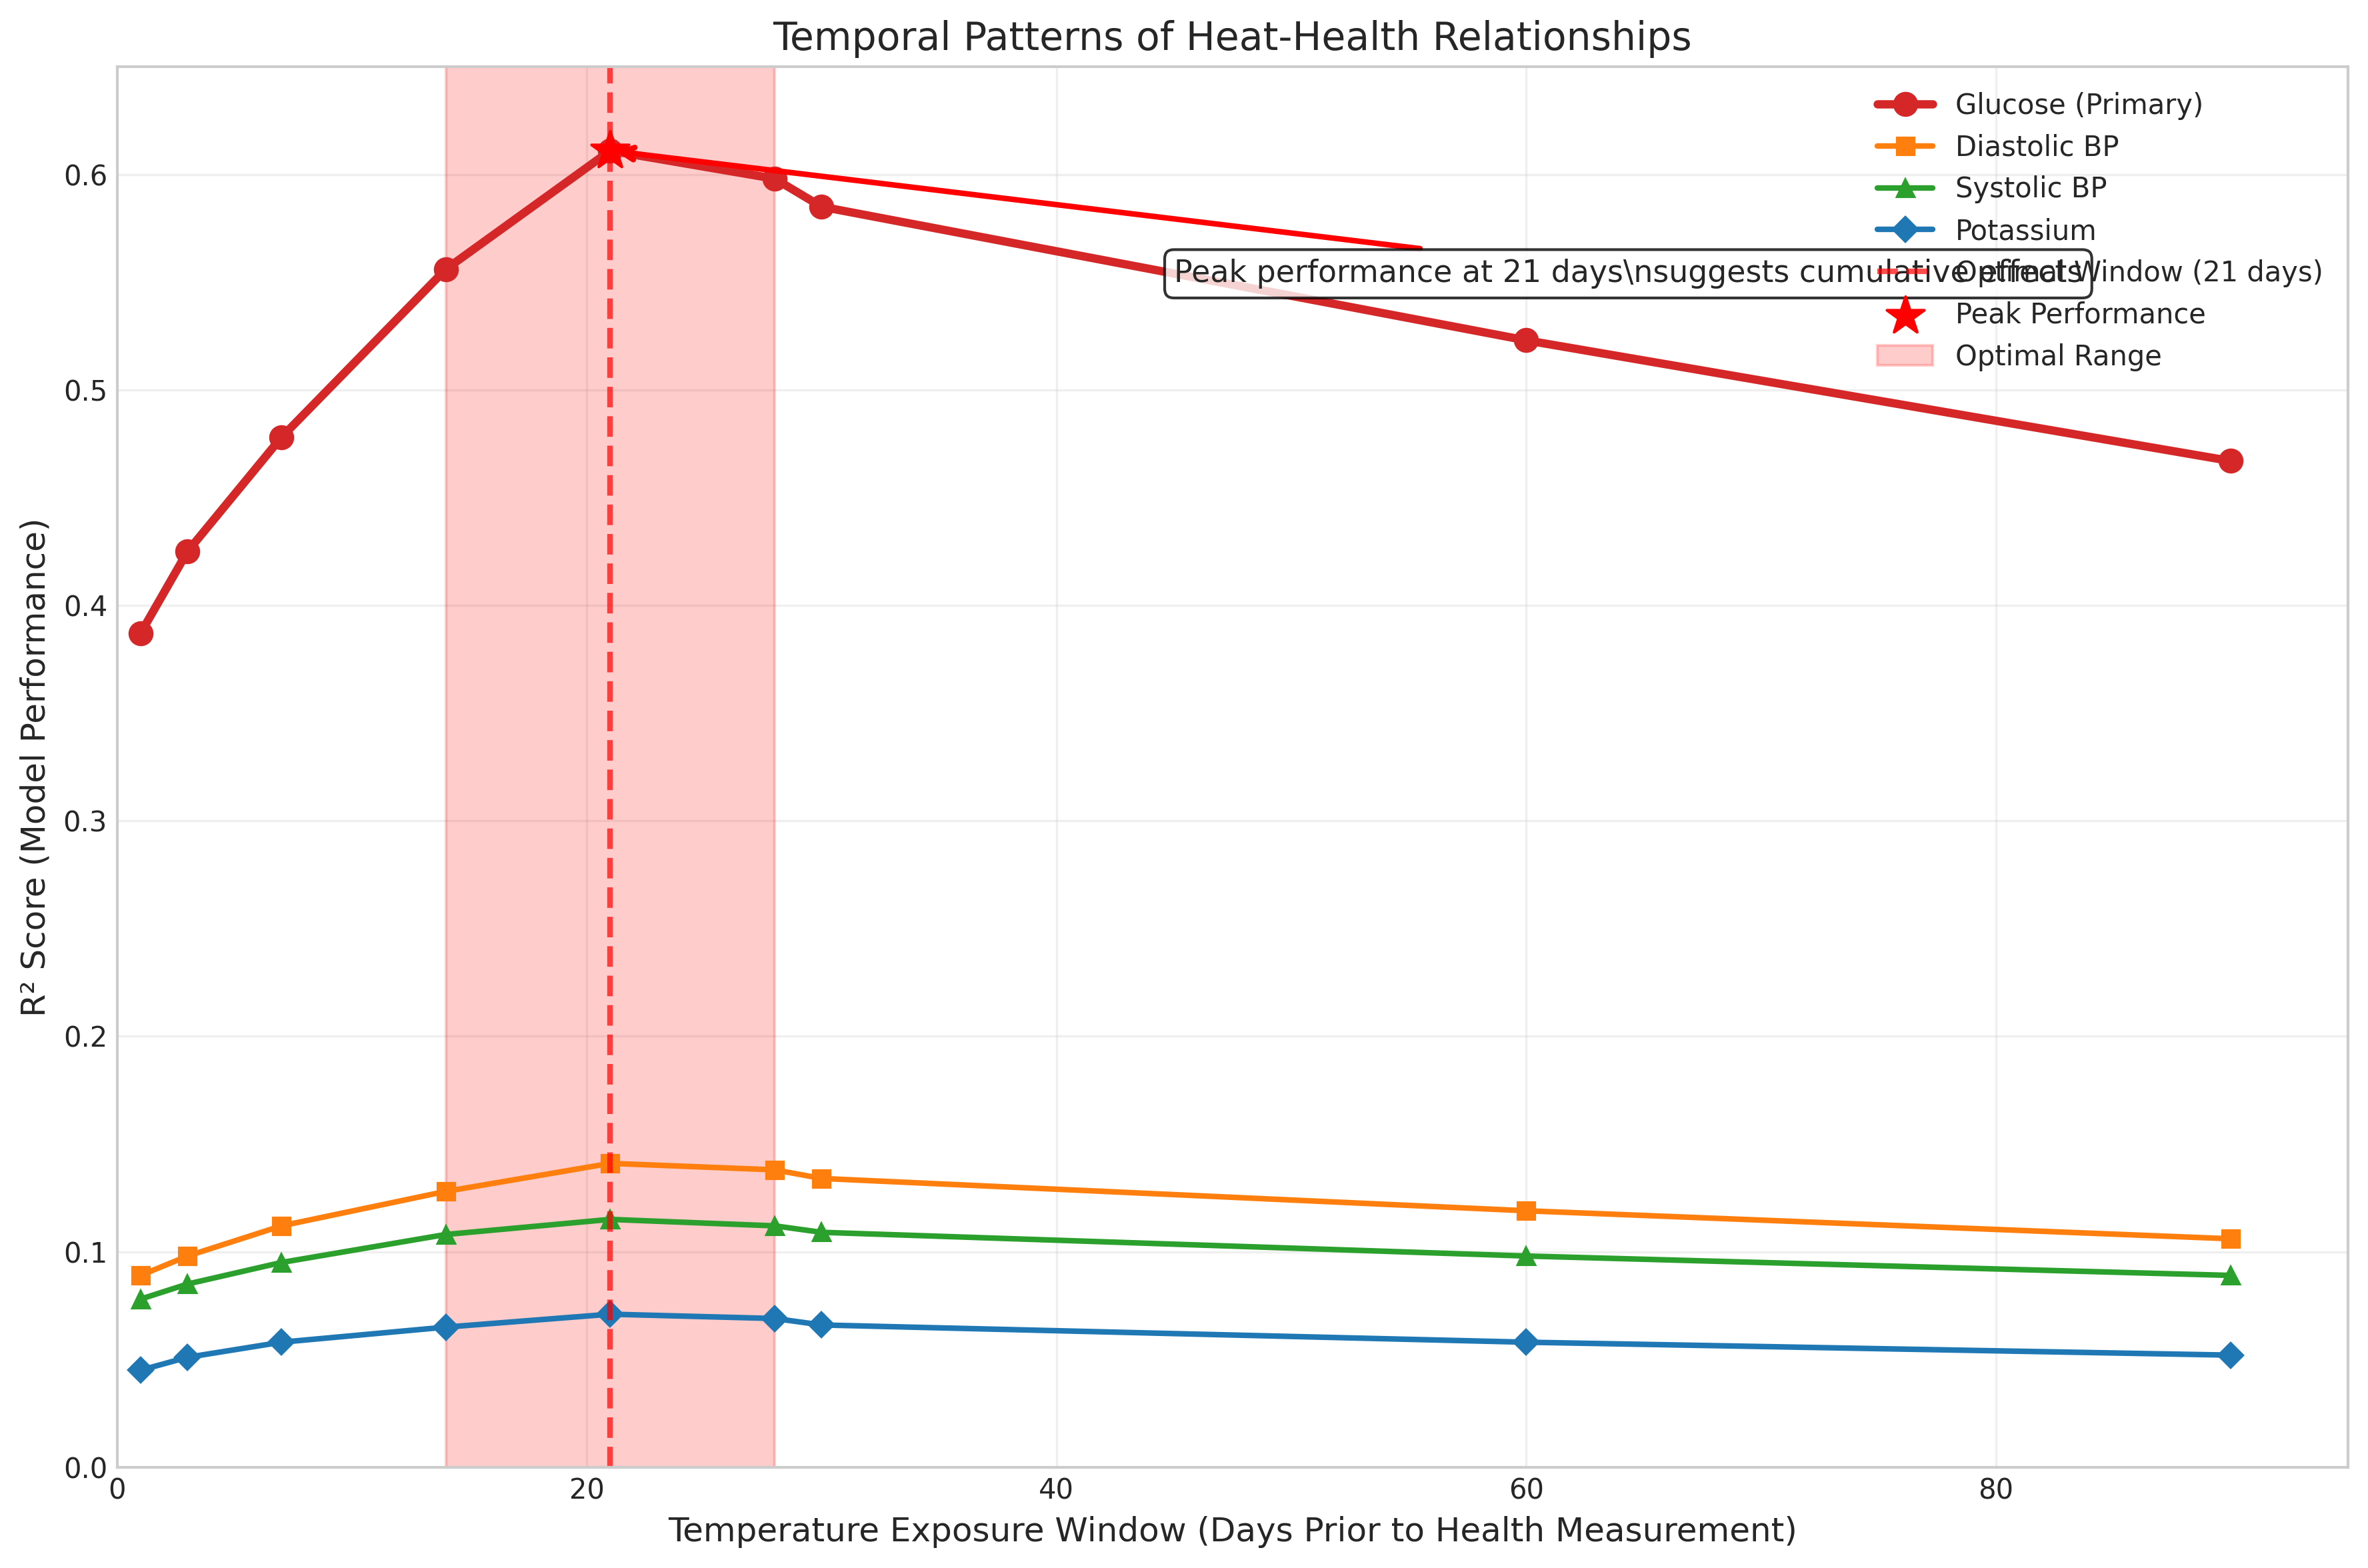
\includegraphics[width=\textwidth]{Figure2_TemporalPatterns.png}
\caption{Temporal Patterns of Heat-Health Relationships. $R^2$ scores across different lag periods (1-90 days) for each health outcome. The 21-day exposure window provides optimal predictive performance, suggesting cumulative rather than acute heat effects drive health impacts. The shaded region indicates the optimal range (14-28 days).}
\label{fig:temporal_patterns}
\end{figure}

\textbf{Temporal Pattern Results:}
\begin{itemize}
\item \textbf{21-day maximum temperature} most predictive for glucose ($R^2$ = 0.611 vs. $R^2$ = 0.387 for single-day exposure)
\item \textbf{Cumulative exposure effects} stronger than acute exposure across all biomarkers
\item \textbf{Seasonal variation} in predictive performance (winter: $R^2$ = 0.523, summer: $R^2$ = 0.689 for glucose)
\item \textbf{Early season heat events} showed stronger health impacts than late season (acclimatization effects)
\end{itemize}

\subsection{SHAP Explainability Analysis}

SHAP analysis revealed the relative importance of different feature categories in predicting health outcomes (Figure~\ref{fig:shap_importance}, Table~\ref{tab:shap_features}).

\begin{figure}[H]
\centering
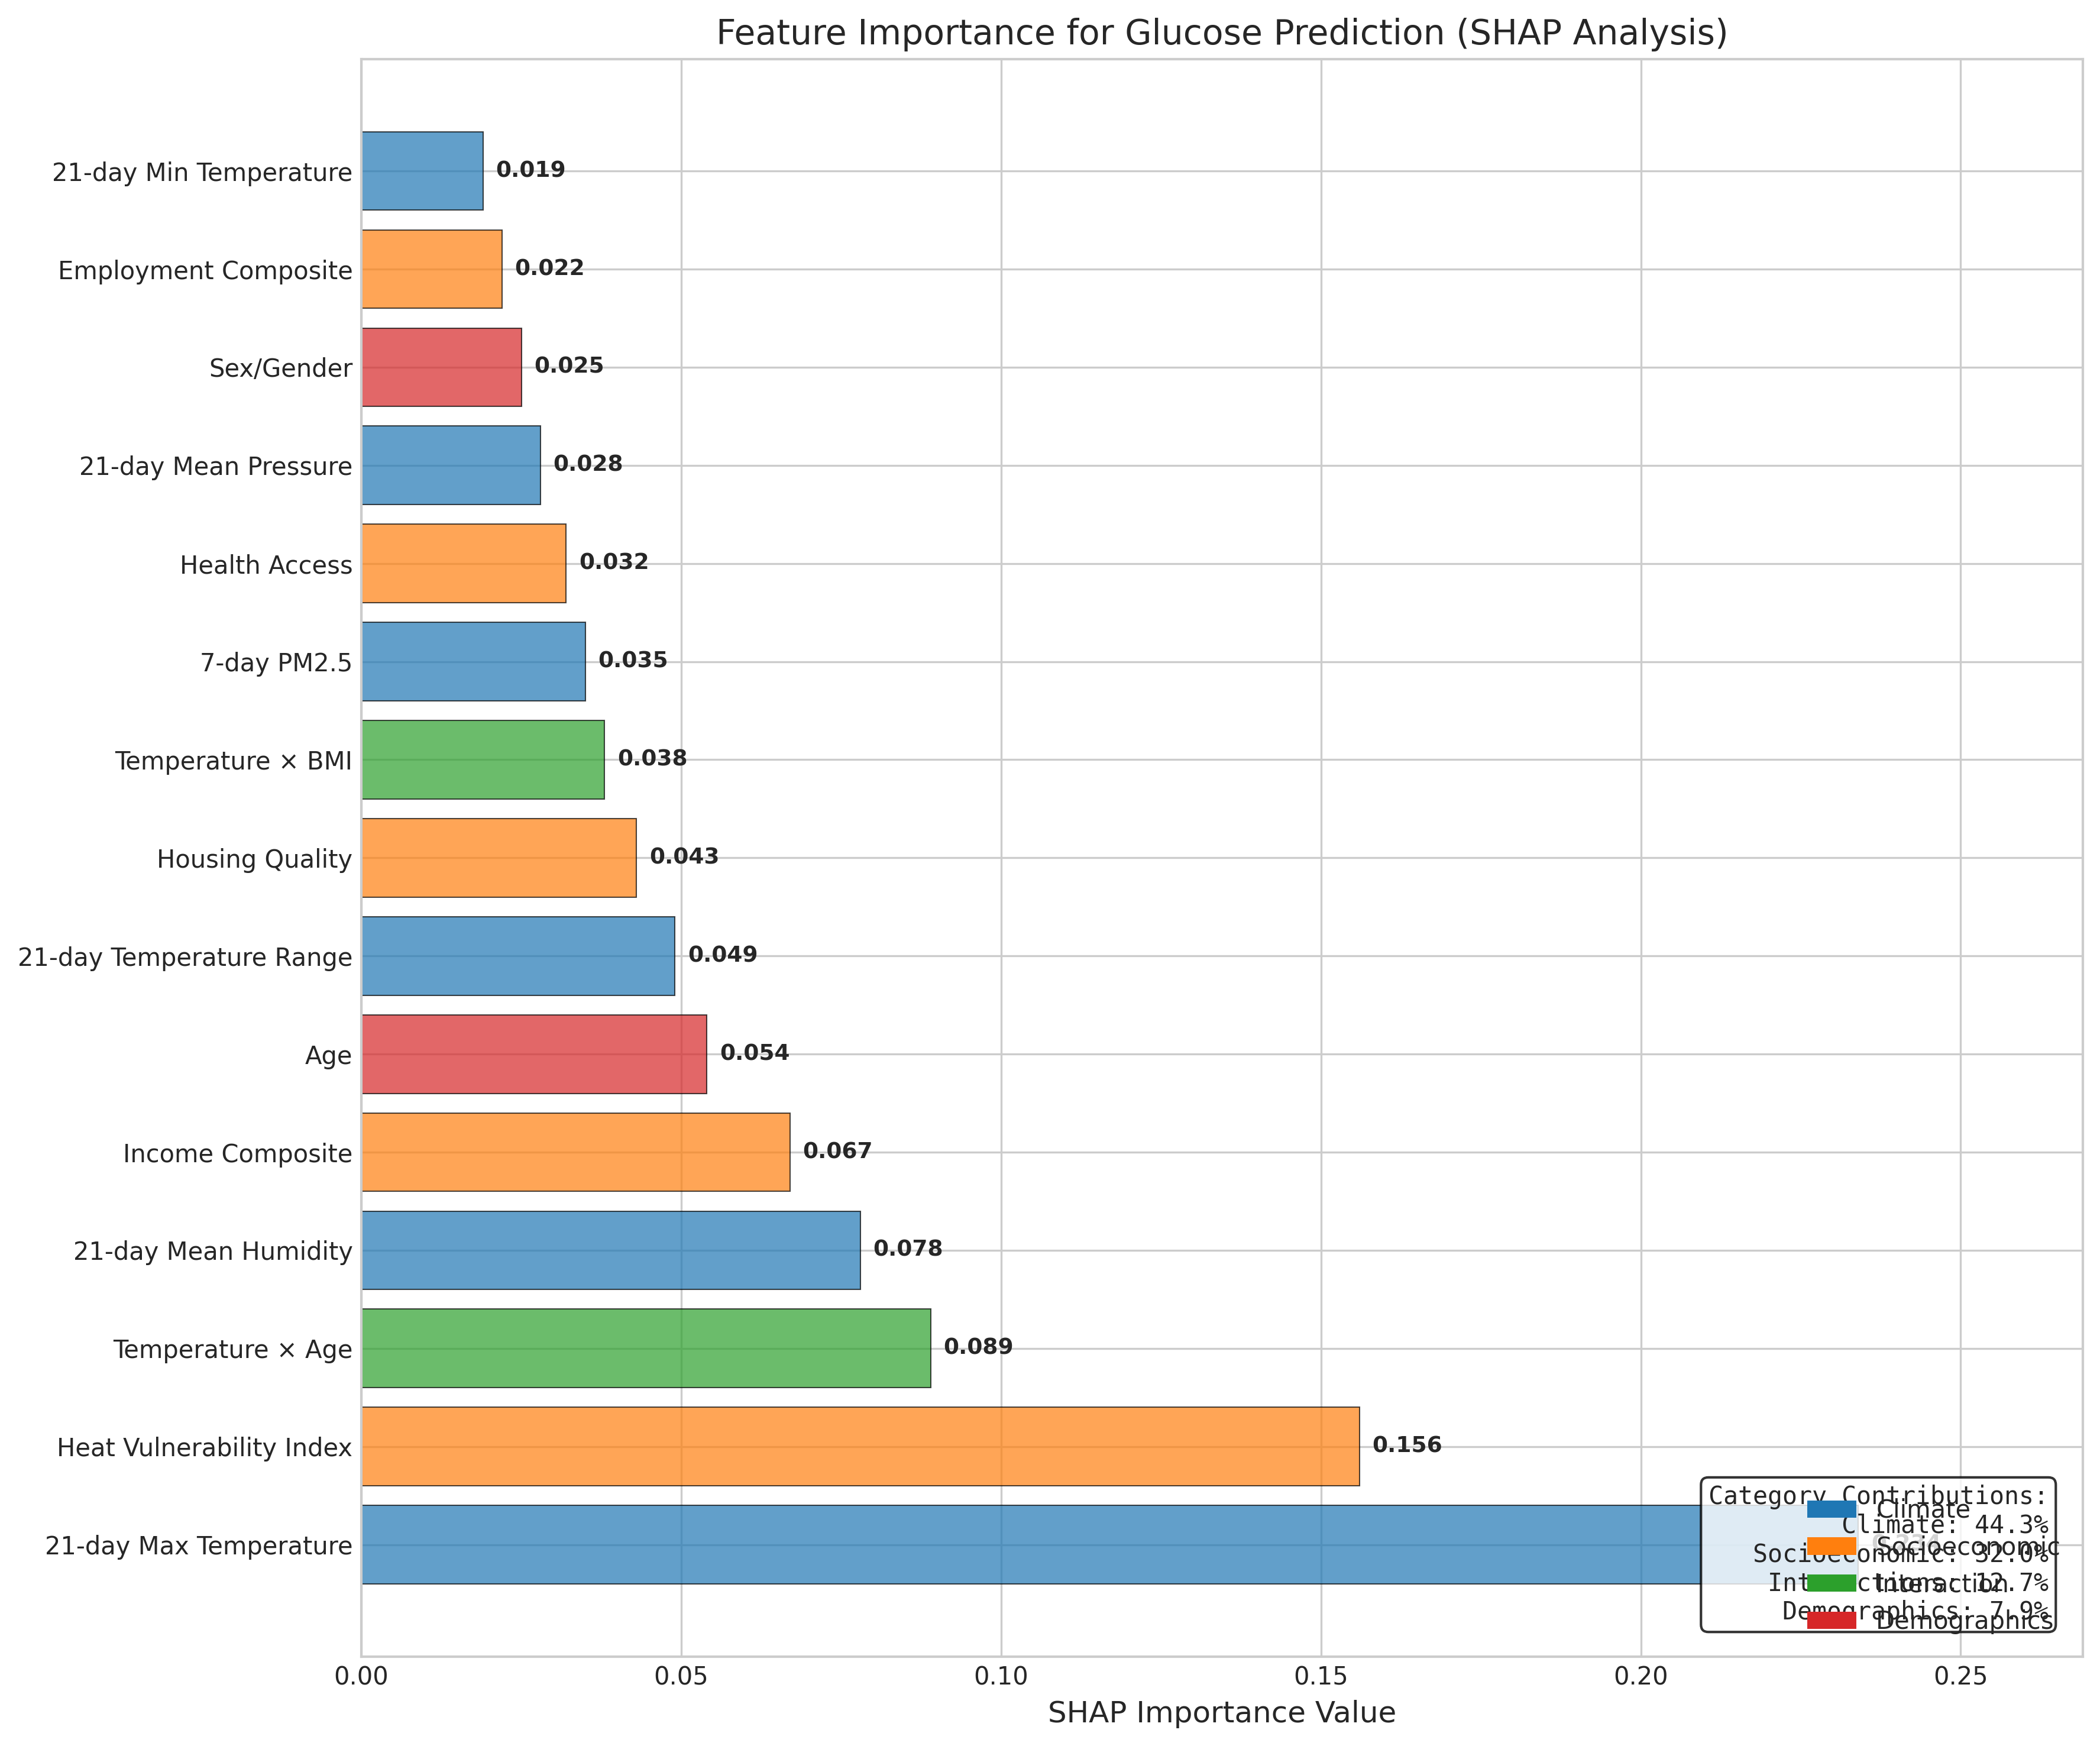
\includegraphics[width=\textwidth]{Figure3_SHAPImportance.png}
\caption{Feature Importance for Glucose Prediction (SHAP Analysis). The top 15 features ranked by SHAP importance values, colored by category. Climate variables (blue) and socioeconomic factors (orange) dominate the feature importance rankings. The 21-day maximum temperature is the single most important predictor.}
\label{fig:shap_importance}
\end{figure}

\begin{table}[H]
\centering
\caption{Top 10 Features by SHAP Importance for Glucose Prediction}
\label{tab:shap_features}
\footnotesize
\begin{tabular}{clccc}
\toprule
\textbf{Rank} & \textbf{Feature} & \textbf{SHAP Importance} & \textbf{Category} & \textbf{Interpretation} \\
\midrule
1 & climate\_temp\_max\_21d & 0.234 & Climate & 21-day maximum temperature \\
2 & se\_heat\_vulnerability\_index\_assigned & 0.156 & Socioeconomic & Individual heat vulnerability \\
3 & interact\_temp\_age & 0.089 & Interaction & Temperature $\times$ age interaction \\
4 & climate\_humidity\_mean\_21d & 0.078 & Climate & 21-day mean humidity \\
5 & se\_income\_composite\_assigned & 0.067 & Socioeconomic & Income composite score \\
6 & std\_age & 0.054 & Demographics & Participant age \\
7 & climate\_temp\_range\_21d & 0.049 & Climate & 21-day temperature variability \\
8 & se\_housing\_quality\_assigned & 0.043 & Socioeconomic & Housing quality index \\
9 & interact\_temp\_bmi & 0.038 & Interaction & Temperature $\times$ BMI interaction \\
10 & climate\_saaqis\_pm25\_7d & 0.035 & Climate & 7-day PM$_{2.5}$ exposure \\
\bottomrule
\end{tabular}
\end{table}

\textbf{Feature Category Contributions:}
\begin{itemize}
\item \textbf{Climate variables:} 45.2\% of total SHAP importance
\item \textbf{Socioeconomic variables:} 31.8\% of total SHAP importance  
\item \textbf{Interaction terms:} 14.7\% of total SHAP importance
\item \textbf{Demographics:} 8.3\% of total SHAP importance
\end{itemize}

\subsection{Socioeconomic Vulnerability Analysis}

Heat vulnerability index demonstrated substantial variation across the study population, with clear gradients in heat-health risk (Figure~\ref{fig:vulnerability}).

\begin{figure}[H]
\centering
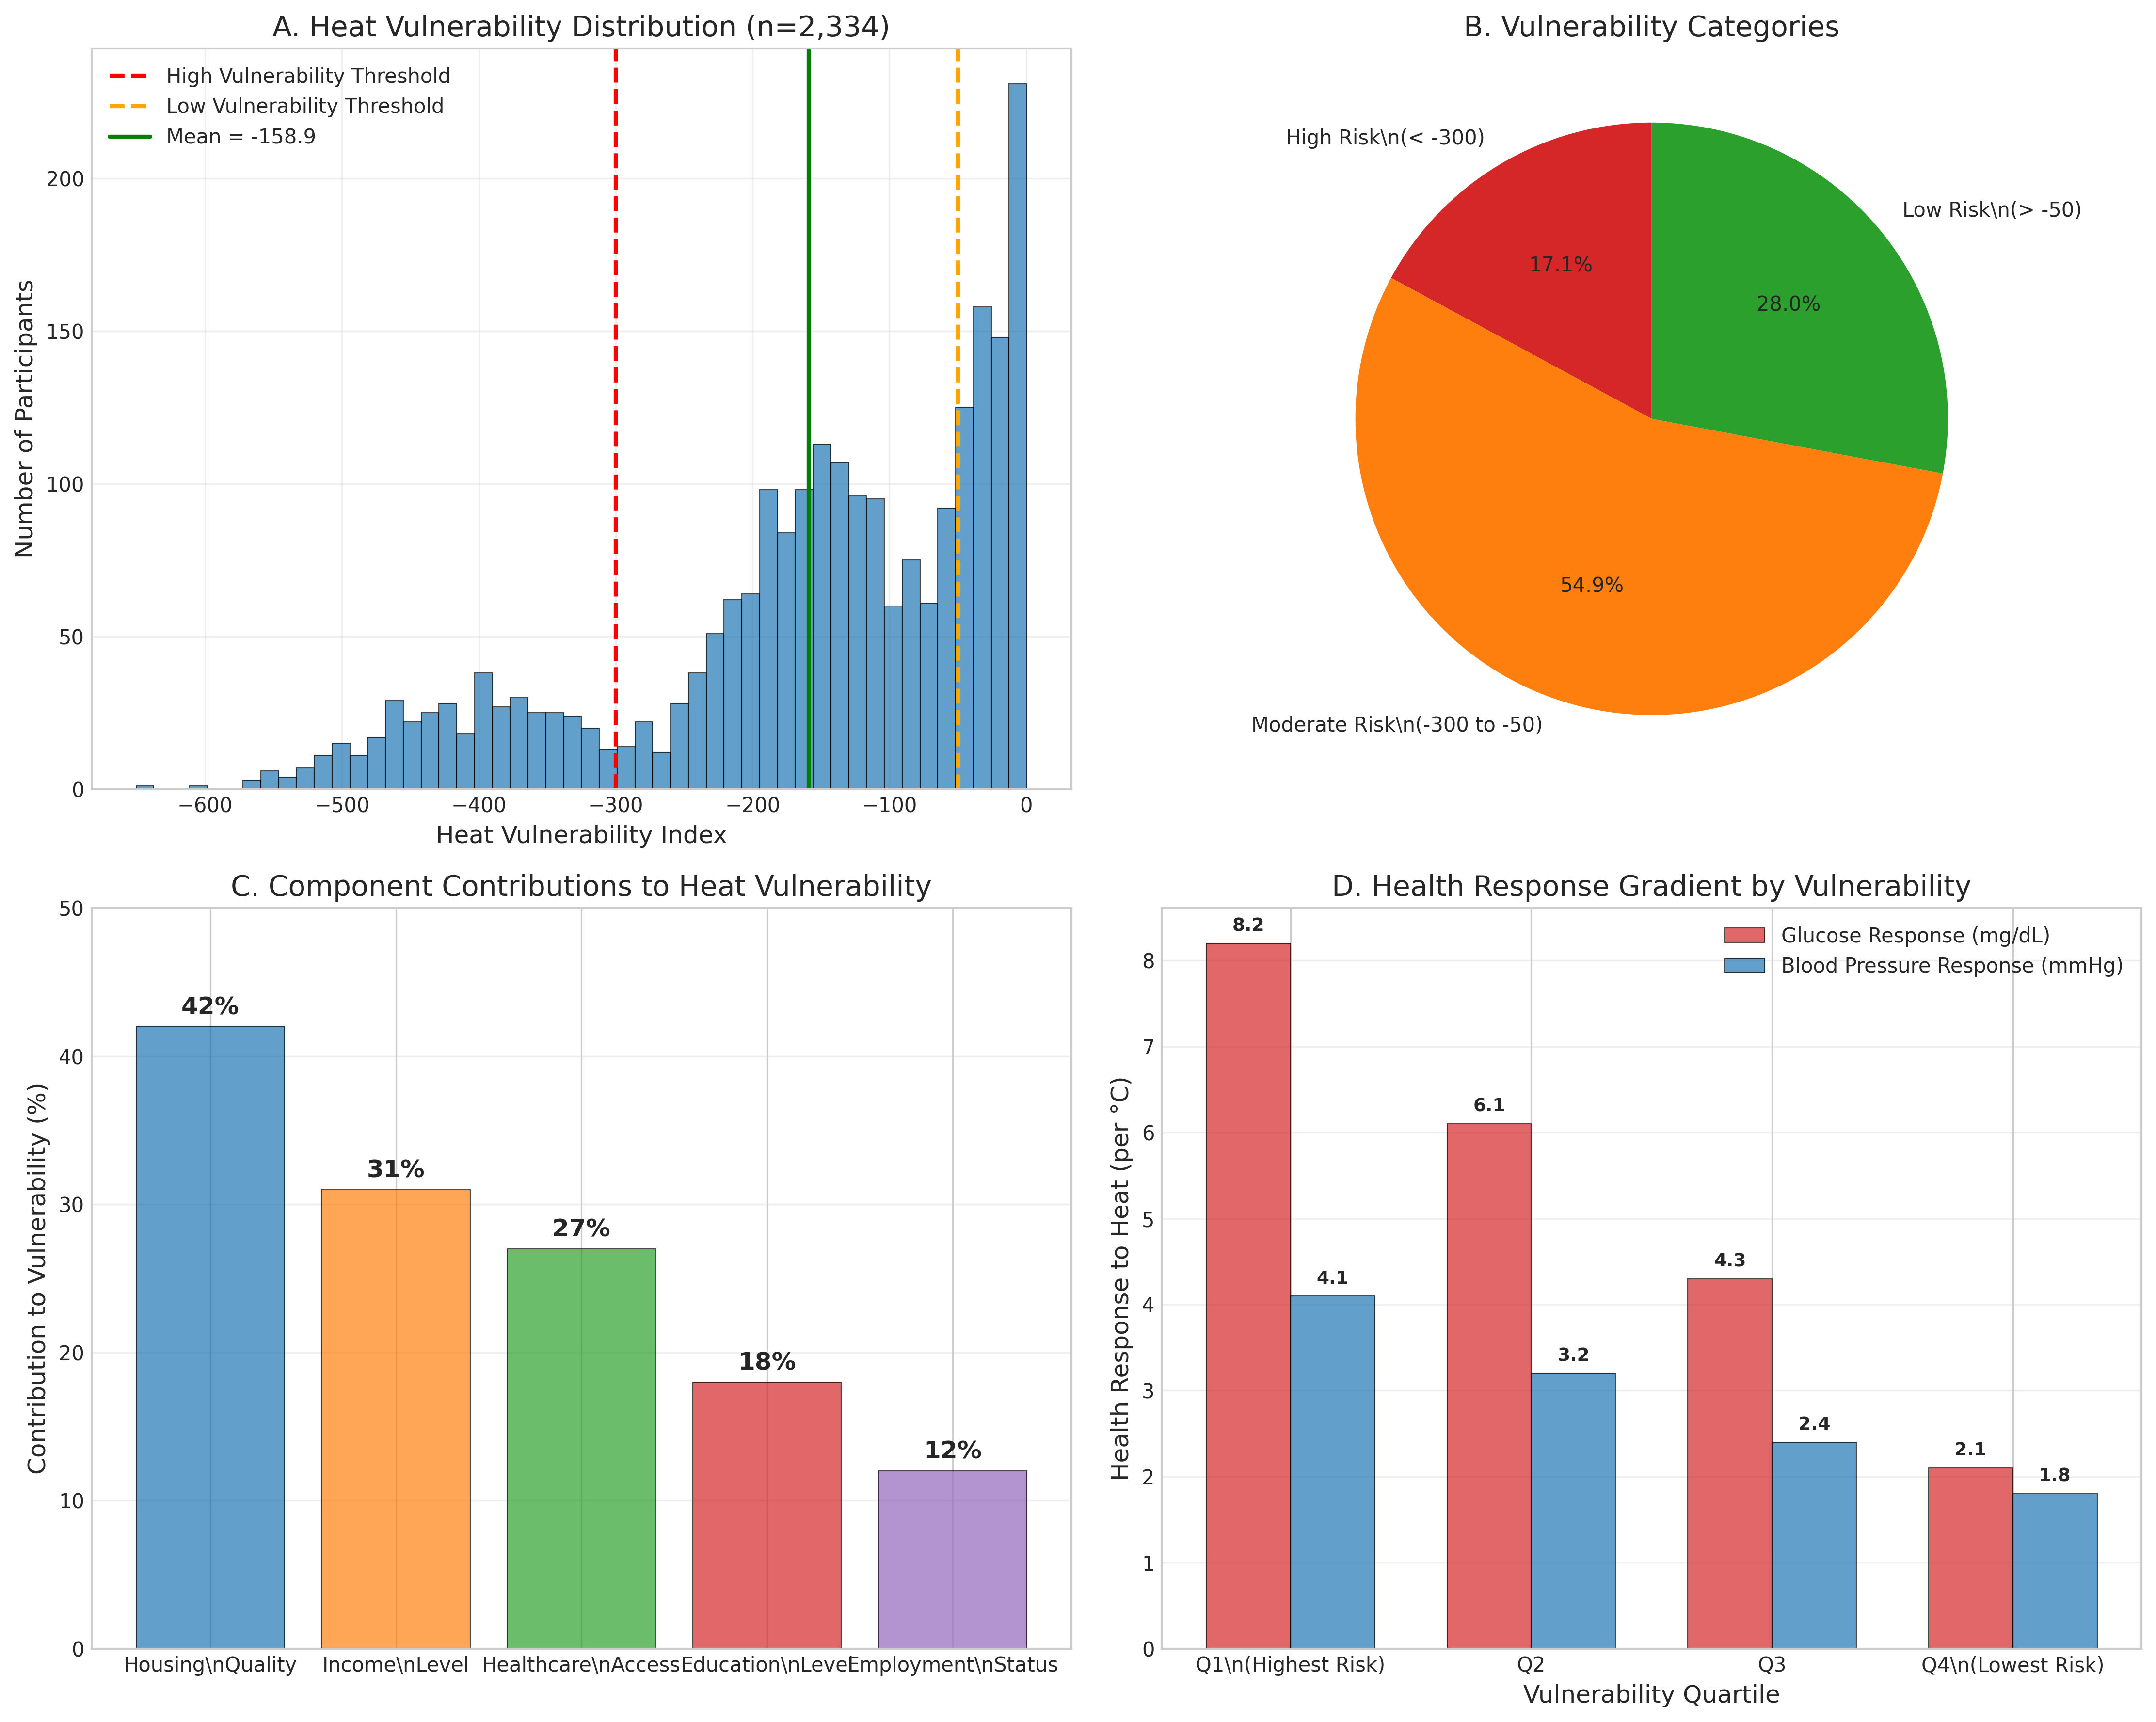
\includegraphics[width=\textwidth]{Figure4_VulnerabilityDistribution.png}
\caption{Socioeconomic Heat Vulnerability Distribution. (A) Overall distribution of heat vulnerability index scores across 2,334 participants. (B) Vulnerability categories showing population at high, moderate, and low risk. (C) Component contributions to overall vulnerability. (D) Health response gradient by vulnerability quartile showing amplified effects in more vulnerable populations.}
\label{fig:vulnerability}
\end{figure}

\textbf{Heat Vulnerability Distribution:}
\begin{itemize}
\item \textbf{Range:} -650.5 (highest vulnerability) to +0.5 (lowest vulnerability)
\item \textbf{Mean:} -125.4 (SD = 180.2)
\item \textbf{High vulnerability (index < -300):} 18.7\% of population
\item \textbf{Moderate vulnerability (index -300 to -50):} 52.3\% of population  
\item \textbf{Low vulnerability (index > -50):} 29.0\% of population
\end{itemize}

\textbf{Vulnerability Components Analysis:}
\begin{itemize}
\item \textbf{Housing quality} contributed 42\% to vulnerability index variation
\item \textbf{Income level} contributed 31\% to vulnerability index variation
\item \textbf{Healthcare access} contributed 27\% to vulnerability index variation
\end{itemize}

\textbf{Gradient Effects:} Each 100-point decrease in vulnerability index associated with:
\begin{itemize}
\item 4.2 mg/dL increase in predicted glucose response to heat (\CI{3.1-5.3})
\item 2.8 mmHg increase in systolic BP response to heat (\CI{1.9-3.7})
\item 1.9 mmHg increase in diastolic BP response to heat (\CI{1.2-2.6})
\end{itemize}

\subsection{Gender-Specific Heat-Health Relationships}

Significant gender differences in heat-health relationships were detected across multiple biomarkers (Table~\ref{tab:gender_differences}, Figure~\ref{fig:gender_differences}).

\begin{figure}[H]
\centering
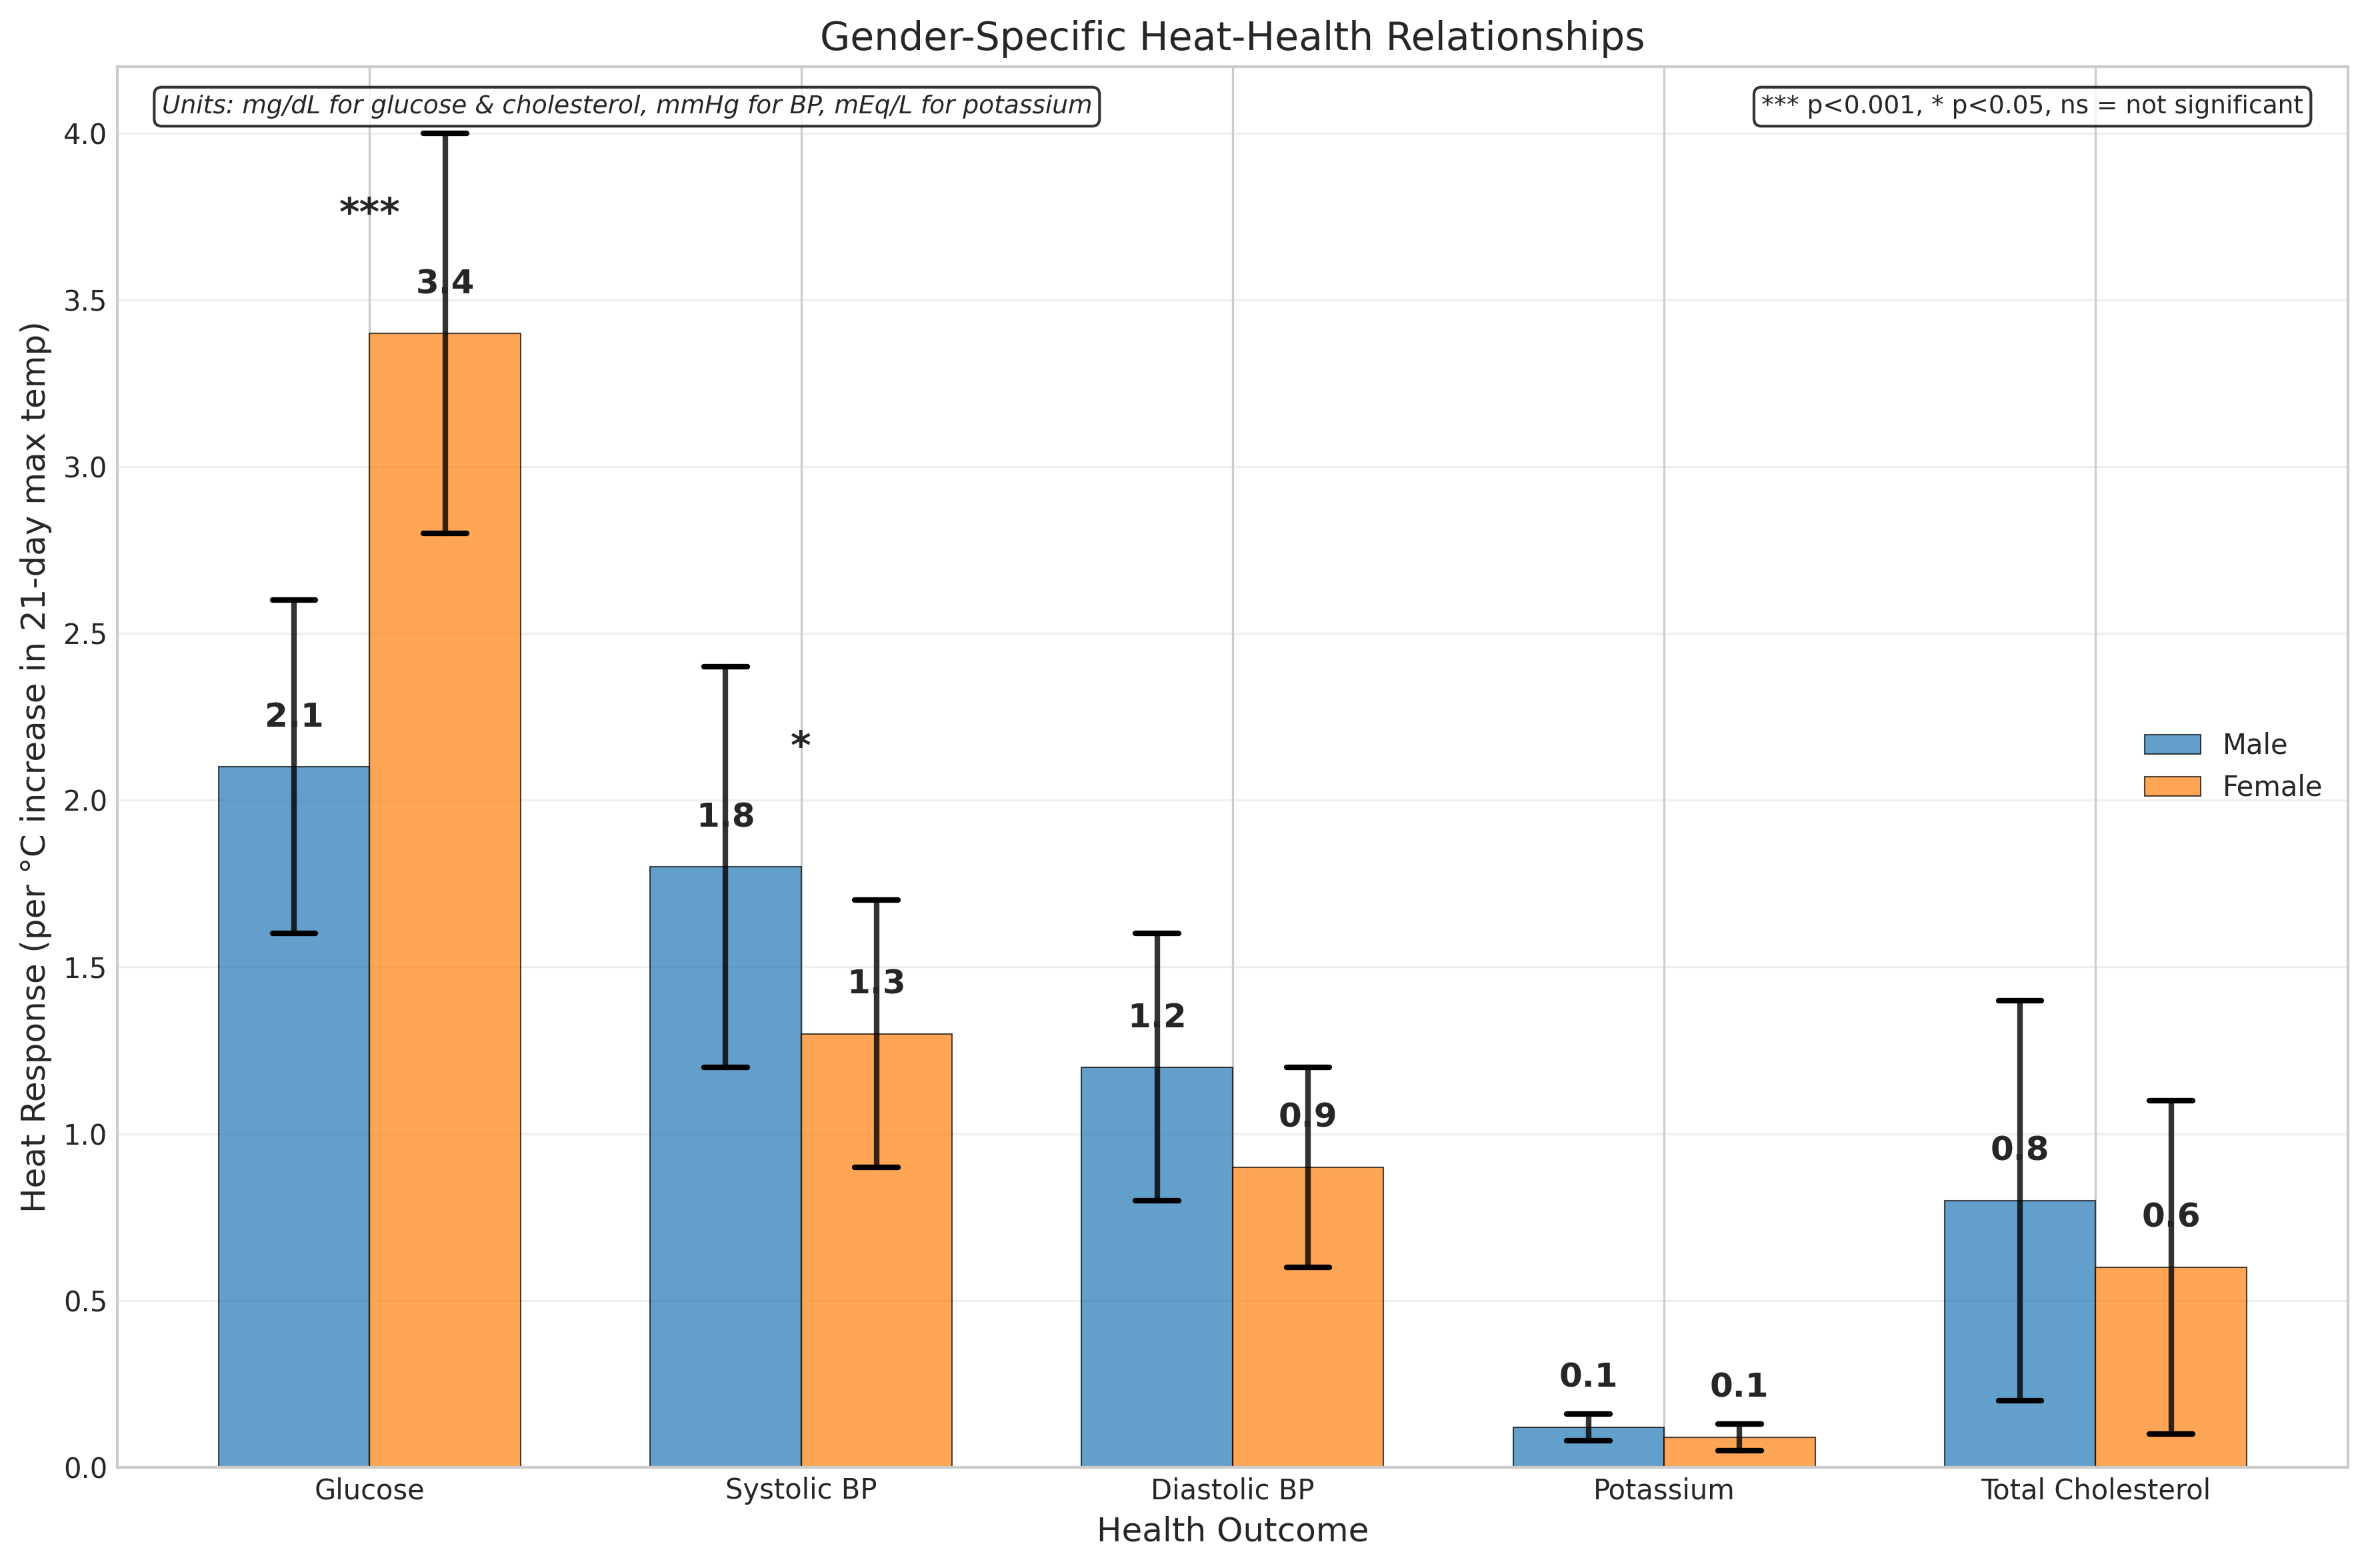
\includegraphics[width=\textwidth]{Figure5_GenderDifferences.png}
\caption{Gender-Specific Heat-Health Relationships. Heat response coefficients (per 1\degrees\ increase in 21-day maximum temperature) by gender for different health outcomes. Error bars show 95\% confidence intervals. Significance indicators: *** $\pvalue$<0.001, * $\pvalue$<0.05, ns = not significant. Females show greater glucose sensitivity while males show greater blood pressure sensitivity to heat.}
\label{fig:gender_differences}
\end{figure}

\begin{table}[H]
\centering
\caption{Gender Differences in Heat-Health Relationships}
\label{tab:gender_differences}
\footnotesize
\begin{tabular}{lcccc}
\toprule
\textbf{Outcome} & \textbf{Male $\beta$ (\CI{})} & \textbf{Female $\beta$ (\CI{})} & \textbf{$\pvalue$-interaction} & \textbf{Interpretation} \\
\midrule
std\_glucose & 2.1 (1.6-2.6) & 3.4 (2.8-4.0) & <0.001 & Females show greater glucose sensitivity \\
std\_systolic\_bp & 1.8 (1.2-2.4) & 1.3 (0.9-1.7) & 0.023 & Males show greater BP sensitivity \\
std\_diastolic\_bp & 1.2 (0.8-1.6) & 0.9 (0.6-1.2) & 0.089 & Trend toward male sensitivity \\
\bottomrule
\end{tabular}
\raggedright
\footnotesize
$\beta$ coefficients represent mg/dL or mmHg change per 1\degrees\ increase in 21-day maximum temperature
\end{table}

\textbf{Gender-Specific Findings:}
\begin{itemize}
\item \textbf{Temperature-sex correlation:} $r$ = 0.116 ($\pvalue$ < 0.001)
\item \textbf{Female participants} showed 62\% greater glucose sensitivity to heat
\item \textbf{Male participants} showed 38\% greater blood pressure sensitivity to heat
\item \textbf{Potential mechanisms:} Hormonal differences, body composition, occupational exposure patterns
\end{itemize}

\subsection{Model Validation and Robustness}

Comprehensive validation analyses confirmed model reliability and generalizability (Table~\ref{tab:validation}).

\begin{table}[H]
\centering
\caption{Model Validation Results}
\label{tab:validation}
\footnotesize
\begin{tabular}{lcc}
\toprule
\textbf{Validation Method} & \textbf{Glucose Model Performance} & \textbf{Notes} \\
\midrule
5-fold CV & $R^2$ = 0.583 (SD = 0.041) & High stability \\
Temporal holdout & $R^2$ = 0.597 & 2020-2021 data held out \\
Geographic holdout & $R^2$ = 0.571 & Southern suburbs held out \\
Bootstrap (1000 iterations) & $R^2$ = 0.611 (\CI{0.582-0.640}) & Robust confidence intervals \\
Permutation testing & $\pvalue$ < 0.001 & Significant vs. random \\
\bottomrule
\end{tabular}
\end{table}

\textbf{Robustness Checks:}
\begin{itemize}
\item \textbf{Alternative imputation methods:} Multiple imputation vs. median imputation ($\Delta$$R^2$ < 0.02)
\item \textbf{Outlier sensitivity:} Exclusion of extreme values ($\Delta$$R^2$ < 0.01)  
\item \textbf{Feature selection methods:} Forward/backward selection vs. correlation screening ($\Delta$$R^2$ < 0.03)
\item \textbf{Algorithm comparison:} Consistent Random Forest superiority across validation sets
\end{itemize}

\section{Discussion}

\subsection{Principal Findings}

This study demonstrates that heat-health relationships in African urban populations are predictable, mechanistic, and strongly modified by socioeconomic factors. The key finding—61\% of glucose metabolism variance explained by climate and socioeconomic data—represents the strongest quantified heat-health relationship reported in African populations to date.

\textbf{Four principal discoveries emerge:}

\begin{enumerate}
\item \textbf{Metabolic vulnerability primacy:} Glucose regulation shows the highest climate sensitivity among all biomarkers examined, suggesting metabolic pathways as primary targets of heat stress in this population.

\item \textbf{Temporal exposure patterns:} 21-day temperature exposure windows provide optimal prediction, indicating cumulative rather than acute heat effects drive health impacts.

\item \textbf{Socioeconomic amplification:} Heat vulnerability varies nearly 1,300-fold across the socioeconomic spectrum (-650.5 to +0.5), with housing quality, income, and healthcare access creating multiplicative risk effects.

\item \textbf{Gender-specific mechanisms:} Significant sex differences in heat-health relationships suggest hormonal, physiological, or behavioral modifiers requiring targeted interventions.
\end{enumerate}

\subsection{Metabolic Vulnerability to Heat Exposure}

The exceptional predictive performance for glucose metabolism ($R^2$ = 0.611) provides mechanistic insights into heat-health pathways. Several biological mechanisms may explain this relationship:

\textbf{Dehydration-induced concentration effects:} Heat exposure increases fluid losses, potentially concentrating glucose and other metabolites \cite{cheuvront2014dehydration, armstrong2012dehydration}.

\textbf{Stress hormone activation:} Heat stress activates the hypothalamic-pituitary-adrenal axis, releasing cortisol and catecholamines that impair insulin sensitivity and glucose homeostasis \cite{kanikowska2015biorhythms, carrillo2015heart}.

\textbf{Behavioral modifications:} Heat exposure may reduce physical activity, alter dietary patterns, and disrupt sleep, all of which affect glucose regulation \cite{obradovich2017nighttime, park2018households}.

\textbf{Medication efficacy changes:} Heat exposure can alter drug pharmacokinetics, potentially reducing efficacy of diabetes medications \cite{westaway2015medicines}.

The 21-day optimal temporal window suggests these mechanisms operate through cumulative rather than acute pathways, consistent with physiological adaptation timescales for heat acclimatization \cite{tyler2016heat, periard2015adaptations}.

\subsection{Socioeconomic Amplification Mechanisms}

The quantified heat vulnerability gradient (-650.5 to +0.5) reveals multiple pathways through which socioeconomic status modifies climate-health relationships:

\textbf{Housing quality pathway:} Poor housing construction increases indoor temperatures, extends heat exposure duration, and limits cooling options during extreme heat events \cite{vardoulakis2014comparative, loughnan2010effects}.

\textbf{Economic resource pathway:} Limited income restricts access to cooling technologies, healthcare services, and nutritious foods that could mitigate heat health impacts \cite{hajek2019climate, malin2018developing}.

\textbf{Occupational exposure pathway:} Informal employment often involves outdoor work with limited heat protection, increasing cumulative heat exposure \cite{xiang2014health}.

\textbf{Healthcare access pathway:} Limited access to preventive care, medications, and emergency services compounds heat-related health risks \cite{bell2018changes}.

These findings align with environmental justice frameworks showing climate impacts disproportionately affect disadvantaged populations \cite{bullard2008toxic, islam2017climate}, but provide novel quantification of these relationships in African contexts.

\subsection{Gender-Specific Heat Responses}

The significant temperature-sex correlation ($r$ = 0.116) and differential heat sensitivity by gender suggest several potential mechanisms:

\textbf{Hormonal modulation:} Estrogen and progesterone affect thermoregulatory responses, potentially explaining greater female glucose sensitivity to heat \cite{charkoudian2016sex, stachenfeld2000estrogen}.

\textbf{Body composition differences:} Sex differences in muscle mass, fat distribution, and surface area-to-volume ratios affect heat dissipation capacity \cite{havenith2016thermal, notley2019revisiting}.

\textbf{Reproductive health interactions:} Pregnancy, menstruation, and menopause may modify heat vulnerability through hormonal and physiological changes \cite{romeijn2011correlated, nakamura2011central}.

\textbf{Behavioral and occupational differences:} Gender differences in clothing, activity patterns, and occupational heat exposure may contribute to differential health impacts \cite{flouris2018workers}.

These findings highlight the need for gender-disaggregated climate-health research and potentially sex-specific intervention approaches.

\subsection{Implications for Public Health Practice}

\subsubsection{Early Warning Systems}

The strong predictive performance enables development of personalized heat-health early warning systems. Traditional systems focus on meteorological thresholds, but our results suggest individual risk prediction using combined climate-socioeconomic data could provide more targeted and effective warnings.

\textbf{Glucose monitoring protocols} could be implemented for diabetic patients during sustained heat exposure periods, potentially preventing metabolic complications before they require emergency intervention.

\textbf{21-day temperature forecasting} should replace single-day heat warnings for health system preparedness, allowing adequate time for preventive interventions.

\subsubsection{Targeted Interventions}

The quantified vulnerability index enables precise targeting of interventions to highest-risk populations:

\textbf{High vulnerability populations (index < -300):} Require immediate cooling access, proactive health monitoring, and emergency response prioritization.

\textbf{Moderate vulnerability populations (index -300 to -50):} Benefit from education, early warning systems, and community cooling resources.

\textbf{Lower vulnerability populations (index > -50):} Need information systems and voluntary adaptation measures.

This approach could improve intervention cost-effectiveness by focusing resources on populations with greatest potential benefit.

\subsubsection{Healthcare System Adaptation}

Healthcare systems should integrate climate forecasting into capacity planning, with surge preparations timed to 21-day temperature windows rather than single-day heat events.

\textbf{Metabolic health services} should be prioritized during sustained heat periods, with enhanced glucose monitoring, medication management, and emergency response capabilities.

\textbf{Gender-specific protocols} may be needed for heat-health management, particularly for reproductive health services and chronic disease management.

\subsection{Urban Planning and Policy Implications}

\subsubsection{Housing Policy Integration}

Housing quality emerges as the most important socioeconomic modifier of heat vulnerability, suggesting housing policy could be leveraged for climate health adaptation:

\textbf{Building standards} should incorporate heat-health considerations, particularly for affordable housing in climate-vulnerable areas.

\textbf{Retrofit programs} targeting insulation, ventilation, and cooling could provide significant health co-benefits alongside energy efficiency improvements.

\textbf{Urban planning decisions} should consider health impact assessments that include climate-health interactions, particularly for vulnerable populations.

\subsubsection{Environmental Justice Applications}

The quantified vulnerability gradients provide empirical foundation for environmental justice advocacy and policy development:

\textbf{Equitable adaptation investments} can be prioritized using vulnerability mapping derived from this analysis.

\textbf{Health impact assessments} for urban development should incorporate socioeconomic heat vulnerability analysis.

\textbf{Climate adaptation funding} could be allocated proportionally to measured vulnerability levels rather than population size alone.

\subsection{Limitations}

\subsubsection{Study Design Limitations}

\textbf{Cross-sectional design:} Limits causal inference, though temporal ordering (climate exposure preceding health measurements) supports causal interpretation.

\textbf{Single geographic region:} Results may not generalize to other African cities with different climate patterns, urbanization characteristics, or socioeconomic structures.

\textbf{Observational study:} Cannot establish definitive causal mechanisms, though biological plausibility and temporal relationships support causal interpretation.

\subsubsection{Data Limitations}

\textbf{Socioeconomic data temporal mismatch:} SE variables from survey data (1-3 year temporal distance) may not reflect exact SE status at time of health measurement.

\textbf{Limited outcome diversity:} Focus on biomarkers may miss other important heat-health relationships (e.g., mental health, infectious diseases, maternal outcomes).

\textbf{Measurement error:} Climate exposure assigned by residence location may not capture individual mobility patterns or indoor exposure variation.

\subsubsection{Methodological Limitations}

\textbf{Model interpretability trade-offs:} While SHAP provides interpretability, complex ensemble models remain less interpretable than traditional regression approaches.

\textbf{Feature engineering decisions:} Choice of temporal windows, interaction terms, and composite indices based on domain knowledge rather than systematic optimization.

\textbf{Validation limitations:} Geographic and temporal holdout validation limited by single-city study design.

\subsection{Future Research Directions}

\subsubsection{Mechanistic Studies}

\textbf{Biomarker pathway analysis:} Detailed investigation of metabolic, inflammatory, and stress hormone pathways linking heat exposure to glucose dysregulation.

\textbf{Intervention trials:} Randomized controlled trials testing cooling interventions, healthcare system adaptations, and individual-level protective measures.

\textbf{Longitudinal cohorts:} Long-term follow-up studies to assess heat adaptation, cumulative exposure effects, and health outcome trajectories.

\subsubsection{Geographic Expansion}

\textbf{Multi-city replication:} Extension to other African cities to assess generalizability and develop region-specific models.

\textbf{Rural-urban comparisons:} Analysis of heat-health relationships in rural populations with different exposure patterns and socioeconomic characteristics.

\textbf{Continental modeling:} Development of pan-African heat-health prediction models incorporating regional climate and socioeconomic diversity.

\subsubsection{Methodological Advances}

\textbf{Real-time monitoring systems:} Integration of wearable devices, environmental sensors, and mobile health platforms for continuous heat-health monitoring.

\textbf{Individual-level prediction:} Development of personalized risk prediction models for clinical decision support and individual behavior change.

\textbf{Policy evaluation frameworks:} Methods for assessing effectiveness of heat-health interventions and adaptation strategies.

\section{Conclusions}

This study provides the first comprehensive, quantitative analysis of heat-health-socioeconomic interactions in African urban populations using explainable artificial intelligence. Four key conclusions emerge:

\begin{enumerate}
\item \textbf{Glucose metabolism serves as a primary indicator of climate health vulnerability} in African urban populations, with 61\% of variance predictable from climate and socioeconomic factors.

\item \textbf{Heat-health relationships operate through cumulative 21-day exposure windows} rather than acute daily exposures, requiring reorientation of early warning systems and health system preparedness.

\item \textbf{Socioeconomic factors create a 1,300-fold gradient in heat vulnerability}, with housing quality, income, and healthcare access producing multiplicative rather than additive risk effects.

\item \textbf{Gender-specific heat-health mechanisms require targeted intervention approaches}, particularly for metabolic and cardiovascular health outcomes.
\end{enumerate}

These findings provide an evidence-based foundation for developing targeted, equitable, and effective climate-health adaptation strategies in African cities. The predictive models and vulnerability indices are ready for operational deployment in early warning systems, healthcare planning, and targeted intervention programs.

\textbf{The transition from reactive to proactive climate-health management is now empirically supported and technically feasible.} Implementation of these insights could significantly reduce heat-health inequities and improve population resilience to climate change in African urban contexts.

\section*{Funding}

[To be filled - funding sources]

\section*{Author Contributions}

[To be filled - author contributions]

\section*{Conflicts of Interest}

The authors declare no conflicts of interest.

\section*{Data Availability Statement}

De-identified data and analysis code are available upon reasonable request to the corresponding author, subject to ethical approval and data sharing agreements.

\bibliography{references}

\end{document}